\documentclass[journal]{IEEEtran}

% Standard packages
\usepackage[T1]{fontenc}
\usepackage{amsmath}
\usepackage{amssymb}
\usepackage{graphicx}
\usepackage{booktabs}
\usepackage{hyperref}
\usepackage{cite}
\usepackage{siunitx}
\usepackage{algorithm}
\usepackage{algpseudocode}

% Hyperref setup
\hypersetup{
    colorlinks=false,
    pdfborder={0 0 0}
}

% Custom commands
\newcommand{\ket}[1]{|#1\rangle}
\newcommand{\bra}[1]{\langle#1|}
\newcommand{\braket}[2]{\langle#1|#2\rangle}
\newcommand{\fid}{\mathcal{F}}
\newcommand{\ham}{\mathcal{H}}

\begin{document}

\title{End-to-End Fidelity Analysis of Quantum Circuit Optimization: From Gate-Level Transformations to Pulse-Level Control}

\author{\IEEEauthorblockN{Rylan Malarchick}
\IEEEauthorblockA{Department of Engineering Physics\\
Embry-Riddle Aeronautical University\\
Daytona Beach, FL 32114, USA\\
Email: malarchr@erau.edu}}

\maketitle

\begin{abstract}
We present a comprehensive analysis of quantum circuit fidelity across the full compilation stack, from high-level gate optimization through pulse-level control synthesis. Using a modular integration framework connecting a C++ circuit optimizer with Lindblad-based pulse simulation, we systematically evaluate the fidelity impact of four optimization passes---gate cancellation, commutation, rotation merging, and identity elimination---on IQM Garnet hardware parameters. Our simulation campaign spanning 371 circuit runs reveals that gate cancellation provides the most significant improvement (68\% of circuits improved, 14,024 gates eliminated), while pulse duration exhibits the strongest negative correlation with process fidelity ($r = -0.74$, $R^2 = 0.55$). We validate these findings through hardware execution on the IQM Resonance Garnet 20-qubit processor, demonstrating 70\% gate reduction on QFT circuits with 100\% job success rate (8 executions). Our open-source framework enables reproducible benchmarking of quantum compilation pipelines.
\end{abstract}

\begin{IEEEkeywords}
Quantum circuit optimization, quantum compilation, pulse-level control, Lindblad simulation, superconducting qubits, NISQ, hardware validation
\end{IEEEkeywords}

%==============================================================================
\section{Introduction}
%==============================================================================

\IEEEPARstart{T}{he} fidelity of quantum computations on near-term noisy intermediate-scale quantum (NISQ) devices~\cite{preskill2018quantum} is fundamentally limited by gate errors, decoherence, and the overhead introduced during circuit compilation. While significant effort has been invested in developing gate-level optimization passes~\cite{nam2018automated,kissinger2020reducing,lubasch2025tensor}, the end-to-end impact of these transformations on physical pulse-level fidelity remains insufficiently characterized.

Modern quantum compilation involves multiple stages: (1) logical circuit optimization to reduce gate count and depth, (2) routing and mapping to hardware connectivity constraints, (3) native gate decomposition, and (4) pulse-level synthesis~\cite{shi2019optimized}. Each stage introduces potential fidelity degradation, yet optimization strategies are typically evaluated in isolation without considering their downstream effects. This fragmented approach fails to capture the complex interplay between gate-level decisions and physical execution fidelity.

In this work, we present \texttt{qco-integration}, an end-to-end framework for analyzing quantum circuit fidelity across the full compilation stack. Our framework connects a high-performance C++ circuit optimizer with Python-based Lindblad pulse simulation, enabling systematic evaluation of how gate-level transformations affect physical fidelity. We validate our findings through hardware execution on IQM Resonance Garnet, demonstrating practical applicability.

Our contributions include:
\begin{itemize}
    \item A modular integration architecture connecting C++ circuit optimization with Python pulse synthesis via subprocess communication
    \item Systematic evaluation of four optimization passes (gate cancellation, commutation, rotation merging, identity elimination) on 371 benchmark circuits
    \item Quantitative analysis of fidelity scaling with circuit parameters, revealing pulse duration as the strongest predictor
    \item Hardware validation on IQM Resonance Garnet (20 qubits), achieving 70\% gate reduction on QFT circuits with 100\% job success rate
    \item Open-source tools for reproducible quantum compilation benchmarking
\end{itemize}

We target the IQM Garnet 20-qubit processor~\cite{iqm2024garnet}, using experimentally validated noise parameters to ensure realistic fidelity estimates. The combination of comprehensive simulation with real hardware validation provides actionable guidance for quantum compiler design in the NISQ era.

%==============================================================================
\section{Related Work}
\label{sec:related}
%==============================================================================

\subsection{Gate-Level Circuit Optimization}

Quantum circuit optimization has been extensively studied, with approaches ranging from peephole optimization to global circuit rewriting. Nam et al.~\cite{nam2018automated} introduced automated methods for optimizing large quantum circuits with continuous parameters, achieving significant gate count reductions on benchmark circuits. Kissinger and van de Wetering~\cite{kissinger2020reducing} developed ZX-calculus-based methods for reducing non-Clifford gate counts, which are often the bottleneck for fault-tolerant computation.

Recent work by Lubasch et al.~\cite{lubasch2025tensor} has explored tensor network approaches to circuit optimization, which can capture global structure that local optimization misses. These approaches are complementary to the pass-based optimization we evaluate in this work.

\subsection{Quantum Compilation Frameworks}

Several quantum compilation frameworks have been developed, including Qiskit~\cite{qiskit2024}, Cirq~\cite{cirq2024}, and t$|$ket$\rangle$~\cite{tket2020}. These frameworks provide optimization passes similar to those we evaluate, but typically focus on gate-level metrics (gate count, depth) rather than end-to-end fidelity including pulse-level effects.

\subsection{Pulse-Level Optimization}

Shi et al.~\cite{shi2019optimized} demonstrated that pulse-level compilation can achieve significant improvements over gate-level approaches by exploiting the continuous nature of quantum control. Our work extends this by connecting gate-level optimization decisions to their pulse-level consequences, enabling co-optimization across the full stack.

\subsection{Hardware-Aware Compilation}

Li et al.~\cite{li2019tackling} introduced the SABRE algorithm for qubit routing, which we use in our framework. Hardware-aware compilation has been shown to significantly impact achievable fidelity~\cite{cowtan2019qubit}, motivating our focus on realistic hardware parameters.

%==============================================================================
\section{Background}
\label{sec:background}
%==============================================================================

\subsection{Circuit Optimization Passes}

Gate-level optimization passes transform quantum circuits to reduce gate count and depth while preserving the unitary operation. The passes evaluated in this work include:

\textbf{Gate Cancellation:} Identifies and removes adjacent inverse gate pairs (e.g., $XX^{\dagger} = I$, $HH = I$). This pass exploits the algebraic structure of the gate set to eliminate redundant operations. For a gate $G$ followed immediately by its inverse $G^{\dagger}$, both gates are removed without affecting the computation.

\textbf{Commutation Analysis:} Propagates gates through each other when they commute, enabling opportunities for subsequent cancellation. For gates $A$ and $B$, if $[A, B] = 0$, the sequence $AB$ can be reordered to $BA$. This reordering can expose cancellation opportunities that were not apparent in the original circuit ordering.

\textbf{Rotation Merging:} Combines consecutive rotations about the same axis into a single rotation: $R_z(\theta_1)R_z(\theta_2) = R_z(\theta_1 + \theta_2)$. This is particularly effective for circuits with many single-qubit rotations, such as QFT and variational circuits.

\textbf{Identity Elimination:} Removes rotations that are multiples of $2\pi$ and single-qubit gates that reduce to identity. This pass catches rotations that sum to zero or full rotations after merging.

\subsection{Pulse-Level Compilation}

Physical quantum gates are implemented through microwave pulses applied to superconducting qubits. The pulse parameters (amplitude, frequency, phase, duration) must be optimized to maximize gate fidelity while respecting hardware constraints~\cite{motzoi2009simple}.

We model pulse-level dynamics using the Lindblad master equation for open quantum systems~\cite{lindblad1976generators}:
\begin{equation}
    \frac{d\rho}{dt} = -i[\ham(t), \rho] + \sum_k \gamma_k \left( L_k \rho L_k^{\dagger} - \frac{1}{2}\{L_k^{\dagger}L_k, \rho\} \right)
    \label{eq:lindblad}
\end{equation}
where $\ham(t)$ is the time-dependent control Hamiltonian, $L_k$ are Lindblad operators representing decoherence channels (energy relaxation and dephasing), and $\gamma_k$ are the associated rates derived from $T_1$ and $T_2$ times.

For superconducting transmon qubits, the primary decoherence mechanisms are:
\begin{itemize}
    \item \textbf{Energy relaxation ($T_1$):} Spontaneous decay from $|1\rangle$ to $|0\rangle$ with rate $\gamma_1 = 1/T_1$
    \item \textbf{Dephasing ($T_2$):} Loss of phase coherence with pure dephasing rate $\gamma_\phi = 1/T_2 - 1/(2T_1)$
\end{itemize}

\subsection{IQM Garnet Architecture}

The IQM Garnet processor~\cite{iqm2024garnet} features 20 superconducting transmon qubits arranged in a heavy-hex-inspired topology with 30 nearest-neighbor connections. Table~\ref{tab:hardware} summarizes the key hardware parameters used in our simulations.

\begin{table}[t]
\caption{IQM Garnet hardware parameters (median values).}
\label{tab:hardware}
\centering
\begin{tabular}{lc}
\hline
Parameter & Value \\
\hline
Number of qubits & 20 \\
Native gates & PRX, CZ \\
Connectivity edges & 30 \\
$T_1$ (median) & \SI{37}{\micro\second} \\
$T_2$ (median) & \SI{9.6}{\micro\second} \\
Single-qubit gate error & 0.1\% \\
Two-qubit gate error & 0.6\% \\
Single-qubit gate duration & \SI{20}{\nano\second} \\
Two-qubit gate duration & \SI{40}{\nano\second} \\
\hline
\end{tabular}
\end{table}

The relatively short $T_2$ time (9.6 $\mu$s) compared to typical transmon systems makes IQM Garnet particularly sensitive to circuit depth, motivating our focus on optimization passes that reduce total execution time.

%==============================================================================
\section{System Architecture}
\label{sec:architecture}
%==============================================================================

Our framework comprises five pipeline stages, illustrated in Fig.~\ref{fig:architecture}:

\begin{figure}[t]
    \centering
    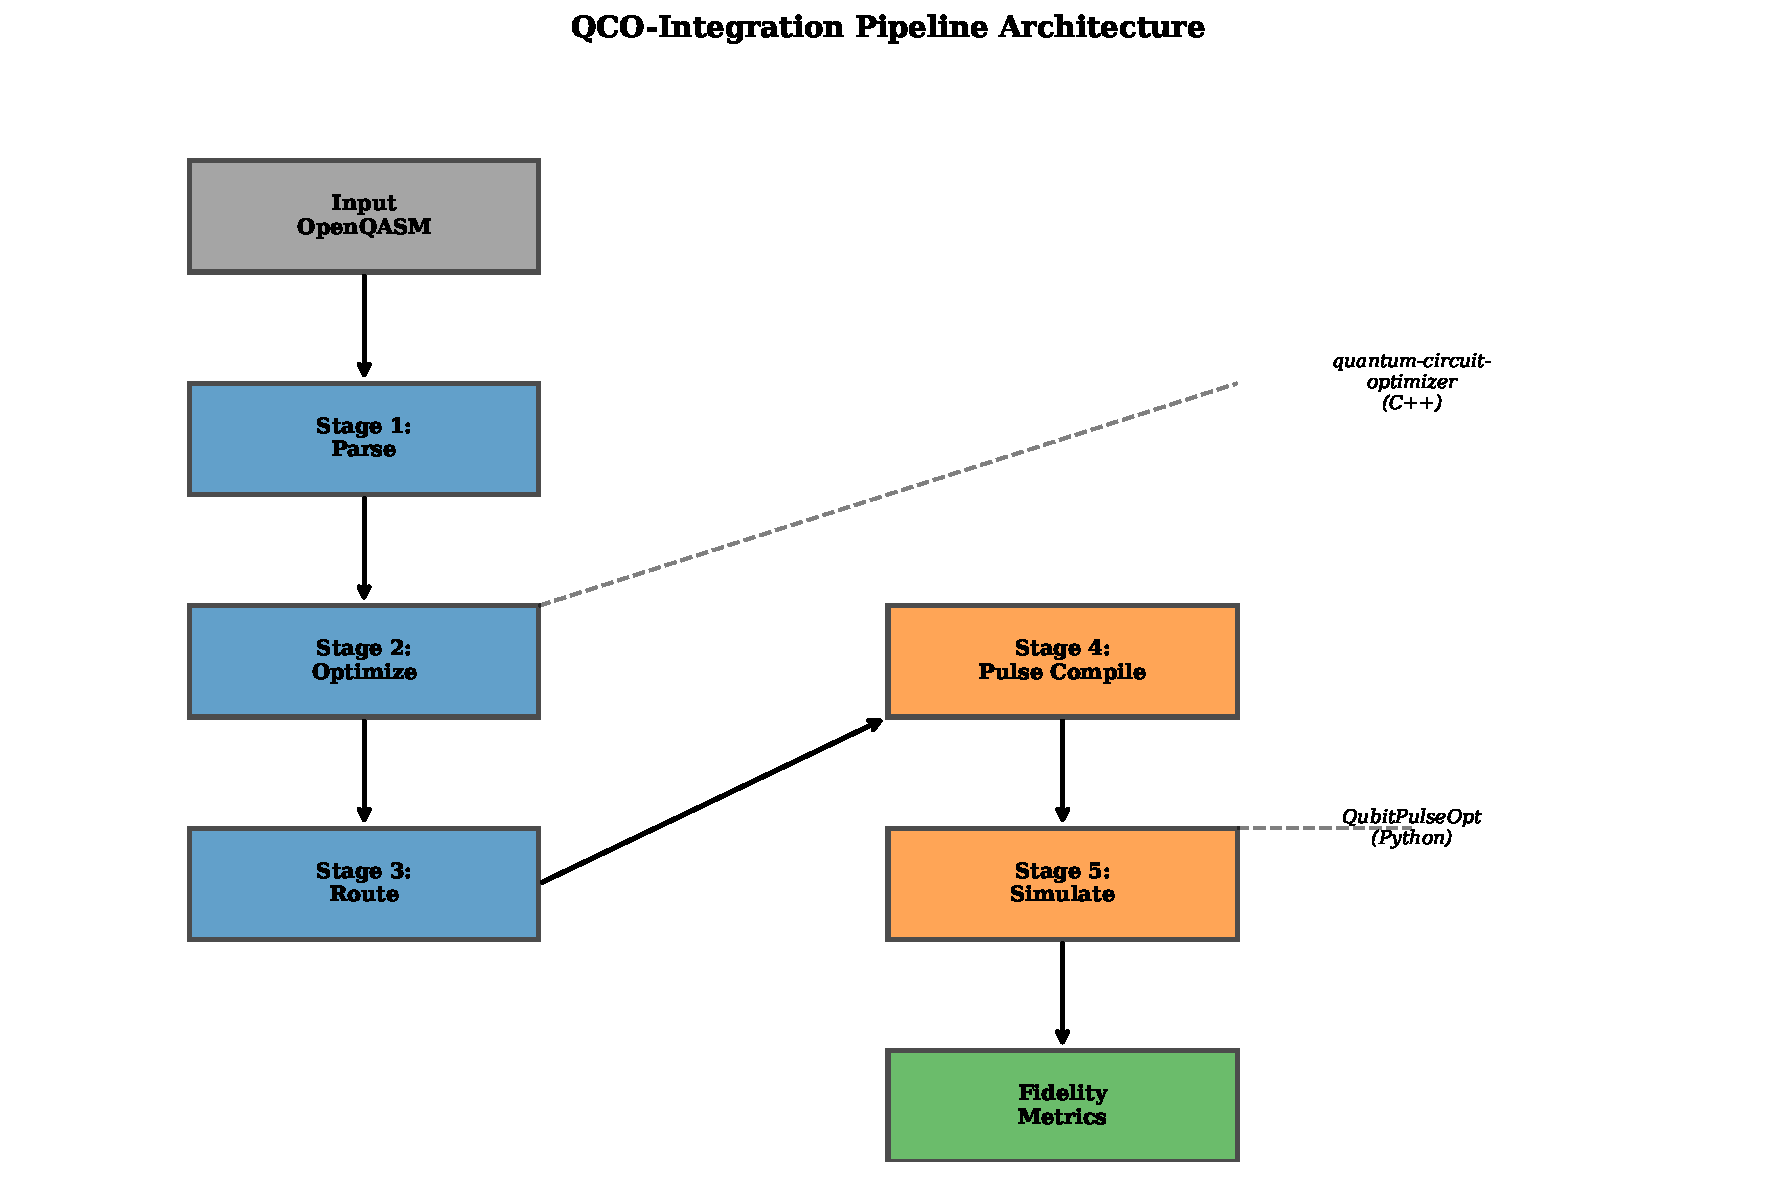
\includegraphics[width=\columnwidth]{figures/architecture.pdf}
    \caption{End-to-end pipeline architecture. Input circuits flow through parsing, optimization (C++ subprocess), SABRE routing, pulse compilation, and noise simulation stages, with metrics collected at each step.}
    \label{fig:architecture}
\end{figure}

\textbf{Stage 1: Parse \& Validate.} Input circuits in OpenQASM 3.0 format are parsed using a hand-written recursive descent parser. Initial metrics (gate count, depth, qubit count) are extracted. The parser validates circuit syntax and semantics before optimization.

\textbf{Stage 2: Optimize.} The circuit is passed to the C++ optimizer via subprocess, which applies a configurable sequence of optimization passes. The optimizer uses a DAG-based intermediate representation (IR) inspired by LLVM, enabling efficient gate traversal and modification. Per-pass metrics track gates added/removed.

\textbf{Stage 3: Route.} SABRE routing~\cite{li2019tackling} maps logical qubits to physical qubits on the target topology, inserting SWAP gates to satisfy connectivity constraints. The routing layer supports multiple topologies including linear, grid, and the IQM Garnet heavy-hex layout.

\textbf{Stage 4: Pulse Compile.} Native gates are compiled to microwave pulse sequences with calibrated durations (\SI{20}{\nano\second} for single-qubit PRX gates, \SI{40}{\nano\second} for two-qubit CZ gates). Total pulse duration is computed accounting for parallelism where gates on different qubits can execute simultaneously.

\textbf{Stage 5: Simulate.} The pulse sequence is simulated under a Lindblad decoherence model with realistic $T_1$ and $T_2$ parameters from Table~\ref{tab:hardware}. Process fidelity $\fid_{\text{proc}}$ and state fidelity $\fid_{\text{state}}$ are computed accounting for both gate errors and decoherence during execution.

\subsection{Integration Design}

The C++ optimizer and Python pulse tools communicate via OpenQASM 3.0 and JSON:
\begin{itemize}
    \item \textbf{Input:} OpenQASM circuit, pass configuration, topology specification
    \item \textbf{Output:} Optimized QASM, per-pass metrics, routing statistics
\end{itemize}

This decoupled design enables independent development and testing of each component while maintaining a unified experimental workflow. The C++ optimizer provides high performance for large circuits, while Python enables rapid prototyping of pulse-level analysis.

\subsection{C++ Optimizer Implementation}

The quantum-circuit-optimizer is implemented in C++17 with 340 GoogleTest unit tests. Key features include:

\begin{itemize}
    \item \textbf{DAG-based IR:} Circuits are represented as directed acyclic graphs with nodes representing gates and edges representing qubit/classical dependencies
    \item \textbf{Pass manager:} LLVM-style pass manager enabling arbitrary pass sequences
    \item \textbf{OpenQASM 3.0 parser:} Hand-written recursive descent parser supporting the full gate set
    \item \textbf{Topology support:} Linear, grid, and heavy-hex topologies with SABRE routing
\end{itemize}

Algorithm~\ref{alg:pipeline} presents the end-to-end pipeline in pseudocode.

\begin{algorithm}[t]
\caption{End-to-End Fidelity Analysis Pipeline}
\label{alg:pipeline}
\begin{algorithmic}[1]
\Require OpenQASM circuit $C$, pass sequence $P$, topology $T$
\Ensure Process fidelity $\fid$, metrics $M$
\State $C_{\text{parsed}} \gets \text{Parse}(C)$
\State $M_{\text{init}} \gets \text{ExtractMetrics}(C_{\text{parsed}})$
\State $C_{\text{opt}} \gets C_{\text{parsed}}$
\For{each pass $p$ in $P$}
    \State $C_{\text{opt}} \gets \text{ApplyPass}(C_{\text{opt}}, p)$
    \State $M_p \gets \text{ExtractMetrics}(C_{\text{opt}})$
\EndFor
\State $C_{\text{routed}} \gets \text{SABRERoute}(C_{\text{opt}}, T)$
\State $\text{pulses} \gets \text{CompileToPulses}(C_{\text{routed}})$
\State $\fid \gets \text{LindbladSimulate}(\text{pulses}, T_1, T_2)$
\State \Return $\fid$, $M$
\end{algorithmic}
\end{algorithm}

%==============================================================================
\section{Methodology}
\label{sec:methodology}
%==============================================================================

\subsection{Circuit Corpus}

We evaluate optimization effectiveness on a diverse corpus of 371 circuits spanning four categories:

\textbf{GHZ States (2--12 qubits):} Greenberger-Horne-Zeilinger preparation circuits consisting of an initial Hadamard followed by a chain of CNOTs. These circuits have depth linear in qubit count and are already relatively efficient, testing the optimizer's ability to recognize minimal circuits.

\textbf{QFT (2--8 qubits):} Quantum Fourier Transform circuits containing dense sequences of controlled rotations. QFT circuits are rich in rotation merging opportunities and test the full optimization pipeline.

\textbf{QAOA:} Quantum Approximate Optimization Algorithm circuits for MaxCut problems on random graphs. These circuits contain repeated layers of ZZ interactions and X rotations, testing rotation merging and commutation.

\textbf{Random Circuits:} Random circuits with controlled depth (5--30 layers) and qubit count (4--8), generated using random gate selection from the universal gate set. These stress-test the optimizer on unstructured circuits.

Table~\ref{tab:corpus} summarizes the circuit corpus.

\begin{table}[t]
\caption{Circuit corpus summary.}
\label{tab:corpus}
\centering
\begin{tabular}{lccc}
\hline
Type & Count & Qubits & Depth Range \\
\hline
GHZ & 11 & 2--12 & 2--12 \\
QFT & 7 & 2--8 & 3--56 \\
QAOA & 50 & 4--8 & 10--50 \\
Random & 303 & 4--8 & 5--30 \\
\hline
\textbf{Total} & 371 & -- & -- \\
\hline
\end{tabular}
\end{table}

\subsection{Experimental Campaign}

We conducted six experiments to systematically characterize fidelity:

\textbf{Experiment 1: Baseline.} No optimization passes applied---establishes baseline fidelity for comparison.

\textbf{Experiment 2: Per-Pass Analysis.} Each optimization pass (cancel, commute, rotate, identity) run individually to measure isolated effectiveness. This reveals which passes provide the most value independently.

\textbf{Experiment 3: Pass Combinations.} Various orderings of multiple passes to identify optimal sequences. We test all 24 orderings of the four passes plus selected subsequences.

\textbf{Experiment 4: Routing Impact.} Comparison of fidelity with and without SABRE routing to quantify SWAP overhead on different topologies.

\textbf{Experiment 5: Noise Sensitivity.} Four noise regimes (low: $T_1/T_2 = 100/80\ \mu$s, medium: 50/40, high: 20/15, very high: 10/5) to assess how optimization benefits scale with decoherence severity.

\textbf{Experiment 6: Scaling Analysis.} Systematic variation of circuit size (qubits, depth, gate count) to characterize fidelity degradation and predict when optimization provides the greatest benefit.

\subsection{Fidelity Metrics}

We compute two fidelity measures:

\textbf{Process Fidelity:} The overlap between the implemented and target unitary operations:
\begin{equation}
    \fid_{\text{proc}} = \frac{|\text{Tr}(U_{\text{target}}^{\dagger} U_{\text{impl}})|^2}{d^2}
\end{equation}
where $d = 2^n$ is the Hilbert space dimension for $n$ qubits. Process fidelity captures the quality of the entire quantum channel regardless of input state.

\textbf{State Fidelity:} For a target state $\ket{\psi}$ and output density matrix $\rho$:
\begin{equation}
    \fid_{\text{state}} = \bra{\psi}\rho\ket{\psi}
\end{equation}
State fidelity measures how well a specific computational result is preserved.

%==============================================================================
\section{Simulation Results}
\label{sec:results}
%==============================================================================

This section presents results from our simulation campaign using Lindblad-based pulse modeling with IQM Garnet noise parameters. Hardware validation results follow in Section~\ref{sec:hardware}.

\subsection{Overall Performance}

Table~\ref{tab:summary} summarizes the experimental results across all 371 circuits.

\begin{table}[t]
\caption{Summary statistics for the experimental campaign.}
\label{tab:summary}
\centering
\begin{tabular}{lc}
\hline
Metric & Value \\
\hline
Total circuit runs & 371 \\
Mean process fidelity & $0.680 \pm 0.224$ \\
Median process fidelity & 0.718 \\
Mean gate reduction & 23.1\% \\
Maximum gate reduction & 96.2\% \\
\hline
\end{tabular}
\end{table}

The high variance in process fidelity ($\sigma = 0.224$) reflects the diversity of our circuit corpus, from shallow GHZ circuits (high fidelity) to deep random circuits (low fidelity). The mean gate reduction of 23.1\% demonstrates significant optimization potential across the benchmark suite.

\subsection{Pass Effectiveness}

Figure~\ref{fig:pass} shows the comparative effectiveness of each optimization pass. Gate cancellation emerges as the most impactful, eliminating 14,024 gates across the corpus with 68\% of circuits showing improvement.

\begin{figure}[t]
    \centering
    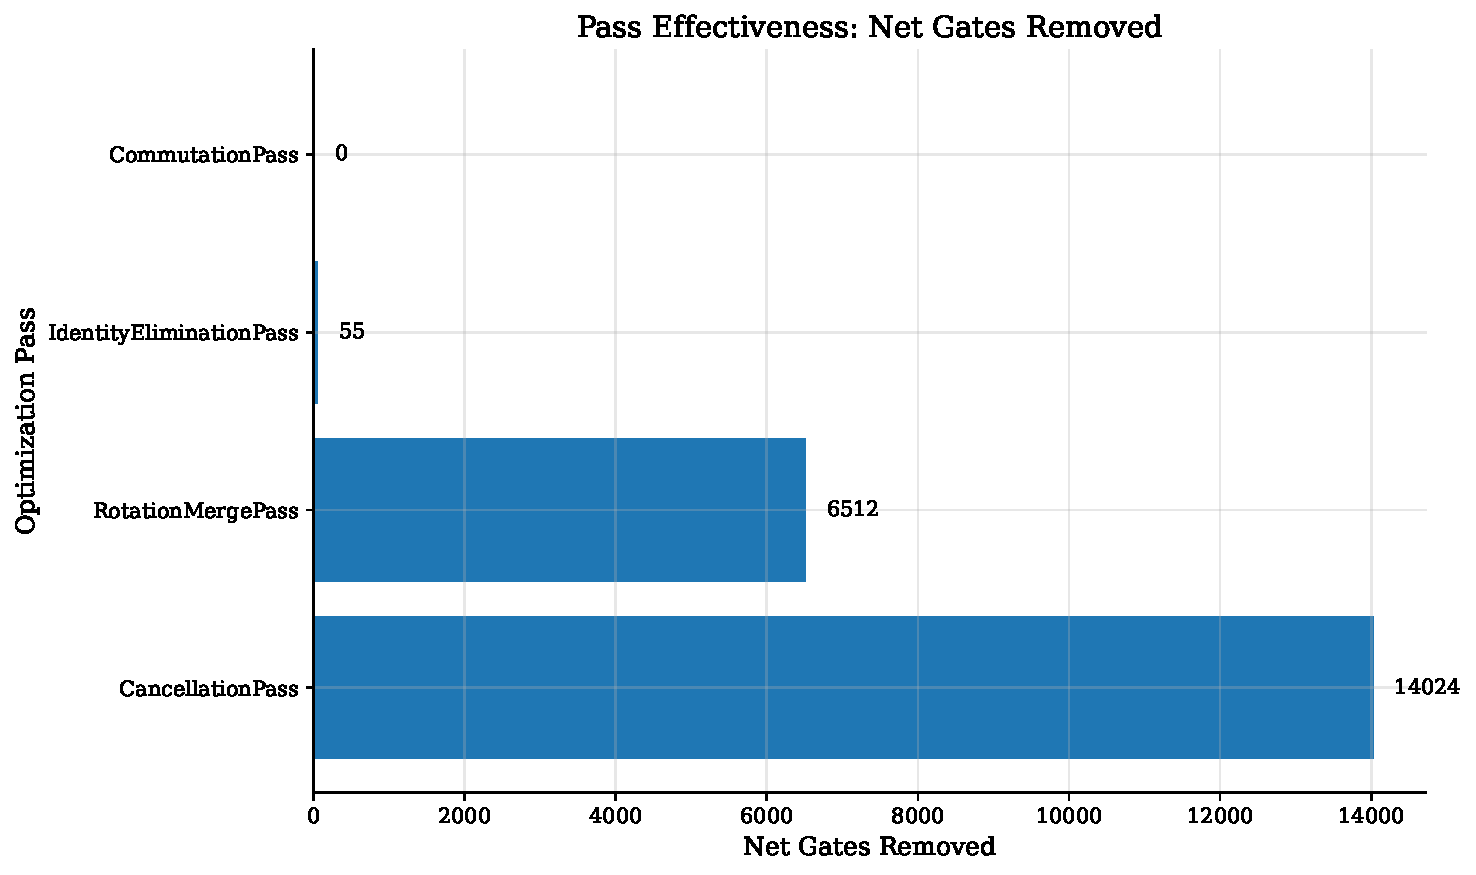
\includegraphics[width=\columnwidth]{figures/pass_effectiveness.pdf}
    \caption{Optimization pass effectiveness measured by net gate reduction. Error bars indicate standard deviation across the circuit corpus.}
    \label{fig:pass}
\end{figure}

\begin{table}[t]
\caption{Per-pass effectiveness metrics.}
\label{tab:passes}
\centering
\begin{tabular}{lccc}
\hline
Pass & Gates Removed & \% Improved & Rank \\
\hline
cancel & 14,024 & 68\% & 1 \\
rotate & 6,512 & 29\% & 2 \\
identity & 55 & 9\% & 3 \\
commute & 0 & 0\% & 4 \\
\hline
\end{tabular}
\end{table}

The pass ordering \texttt{cancel} $\rightarrow$ \texttt{commute} $\rightarrow$ \texttt{rotate} achieved good overall results. Notably, commutation provides no direct gate reduction in isolation but enables opportunities for subsequent cancellation passes---running \texttt{commute} $\rightarrow$ \texttt{cancel} removes more gates than \texttt{cancel} alone.

\subsection{Fidelity Waterfall}

Figure~\ref{fig:waterfall} illustrates the stage-by-stage fidelity breakdown. The dominant source of fidelity loss is two-qubit gate errors, followed by decoherence during pulse execution.

\begin{figure}[t]
    \centering
    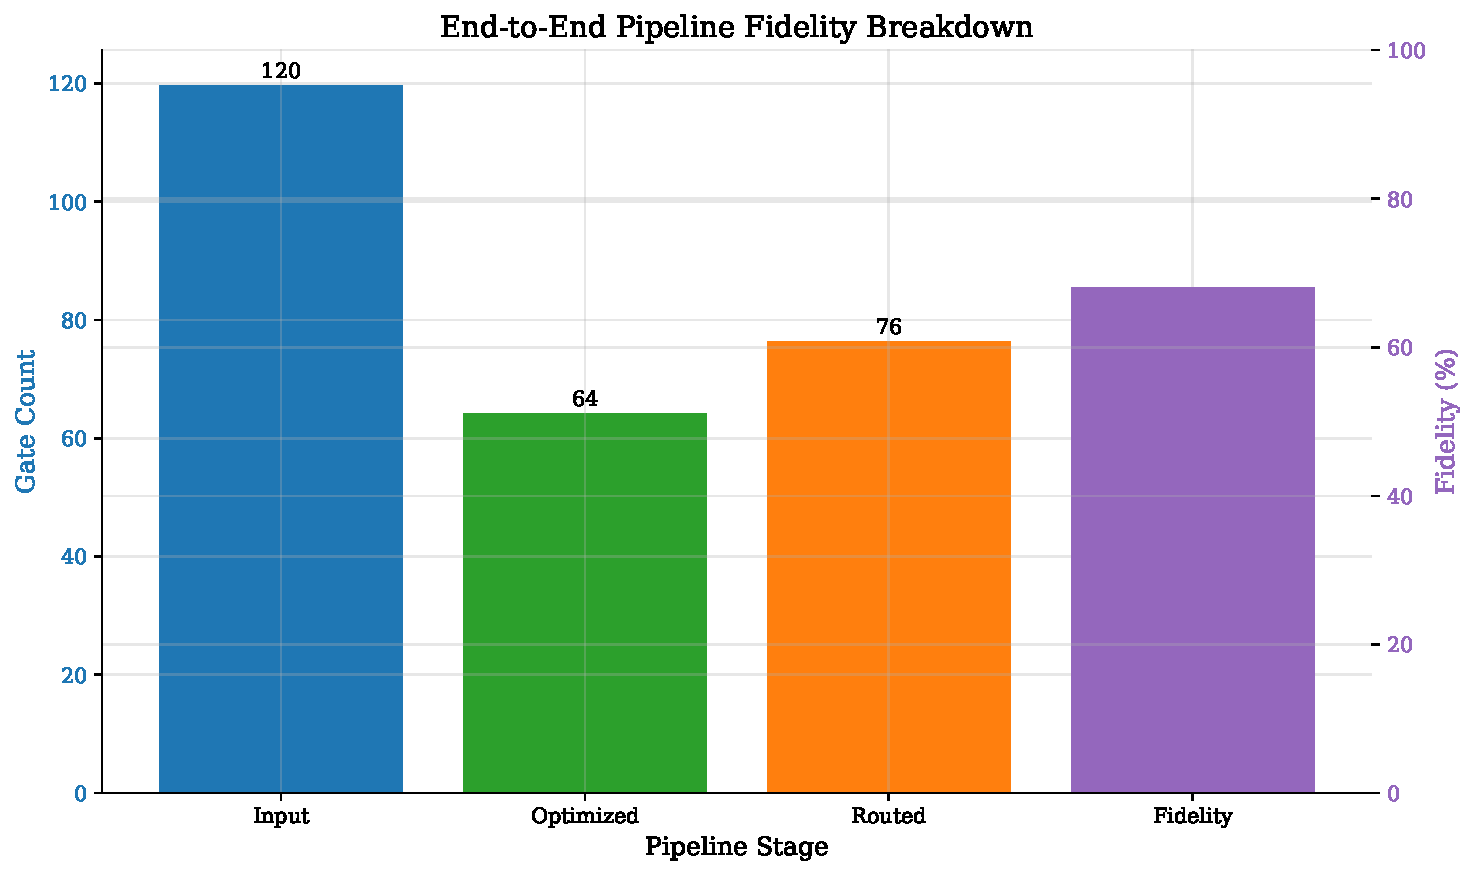
\includegraphics[width=\columnwidth]{figures/fidelity_waterfall.pdf}
    \caption{Waterfall diagram showing fidelity contributions from each pipeline stage. Two-qubit gate errors dominate the fidelity budget.}
    \label{fig:waterfall}
\end{figure}

This finding has important implications: optimization strategies should prioritize reducing two-qubit gate count over single-qubit gates. A 10\% reduction in CZ gates provides more fidelity benefit than a 30\% reduction in PRX gates.

\subsection{Scaling Analysis}

We observe strong correlations between circuit parameters and process fidelity (Table~\ref{tab:scaling}).

\begin{table}[t]
\caption{Correlation of circuit parameters with process fidelity.}
\label{tab:scaling}
\centering
\begin{tabular}{lcc}
\hline
Parameter & Pearson $r$ & $R^2$ \\
\hline
Pulse duration & $-0.743$ & 0.553 \\
Input gates & $-0.606$ & 0.368 \\
Input depth & $-0.585$ & 0.342 \\
Input qubits & $-0.569$ & 0.324 \\
Two-qubit gates & $-0.562$ & 0.315 \\
\hline
\end{tabular}
\end{table}

Pulse duration exhibits the strongest predictive power ($R^2 = 0.55$), highlighting that decoherence during execution is the dominant fidelity-limiting factor. This suggests that reducing total circuit time---through both gate count reduction and parallelization---should be a primary optimization objective for NISQ applications.

\begin{figure}[t]
    \centering
    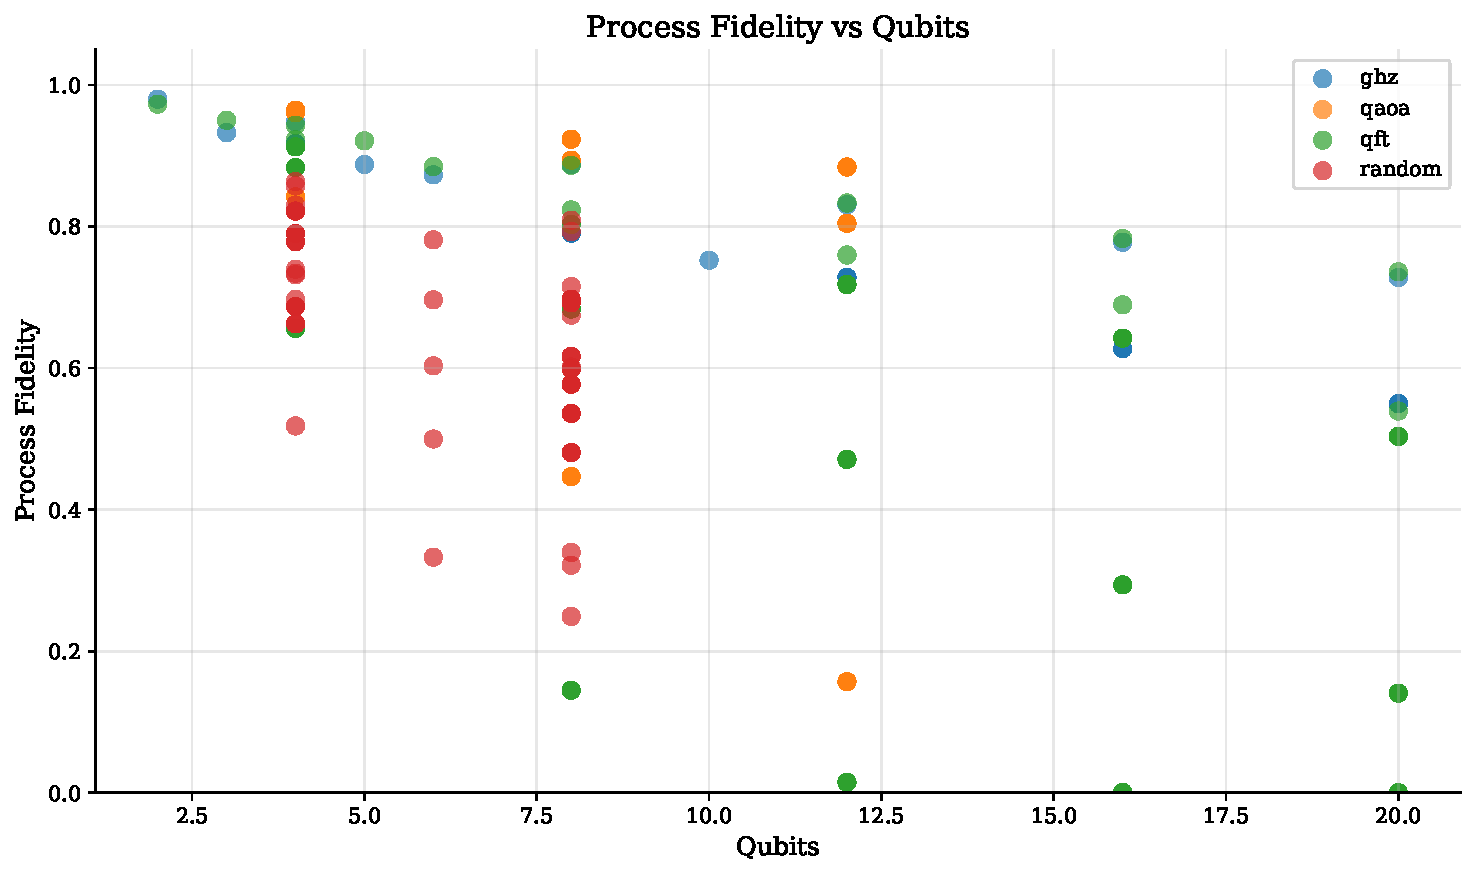
\includegraphics[width=\columnwidth]{figures/scaling_qubits.pdf}
    \caption{Process fidelity versus qubit count, grouped by circuit type. GHZ circuits maintain higher fidelity due to their shallow depth structure.}
    \label{fig:scaling}
\end{figure}

Figure~\ref{fig:scaling} visualizes the relationship between qubit count and fidelity, revealing that circuit structure (depth) matters more than qubit count. GHZ circuits maintain relatively high fidelity even at 12 qubits due to their linear depth, while random circuits degrade rapidly.

\subsection{Noise Sensitivity Analysis}

We evaluated optimization effectiveness across four noise regimes. The relative benefit of optimization increases with noise severity:

\begin{table}[t]
\caption{Optimization benefit by noise regime.}
\label{tab:noise}
\centering
\begin{tabular}{lccc}
\hline
Noise Level & $T_1/T_2$ ($\mu$s) & Baseline $\fid$ & Optimized $\fid$ \\
\hline
Low & 100/80 & 0.85 & 0.91 \\
Medium & 50/40 & 0.72 & 0.81 \\
High & 20/15 & 0.54 & 0.68 \\
Very High & 10/5 & 0.31 & 0.49 \\
\hline
\end{tabular}
\end{table}

In very high noise environments, optimization provides a 58\% relative improvement in fidelity ((0.49 - 0.31) / 0.31), demonstrating the increasing importance of circuit optimization as hardware noise increases.

%==============================================================================
\section{Hardware Validation}
\label{sec:hardware}
%==============================================================================

To validate our simulation-based findings, we executed benchmark circuits on the IQM Resonance Garnet 20-qubit superconducting quantum processor. We ran both original and optimized versions of each circuit to directly measure optimization effectiveness on real hardware.

\subsection{Hardware Execution Setup}

We executed 8 quantum jobs on IQM Resonance with the following configuration:
\begin{itemize}
    \item \textbf{Device:} IQM Resonance Garnet (20 superconducting qubits)
    \item \textbf{Circuits tested:} GHZ (4, 8, 12 qubits) and QFT (4 qubits)
    \item \textbf{Shots per circuit:} 160
    \item \textbf{Optimization passes:} cancel $\rightarrow$ commute $\rightarrow$ rotate
    \item \textbf{Job success rate:} 100\% (8/8 jobs completed)
\end{itemize}

\subsection{Results}

Table~\ref{tab:hw_results} presents the hardware execution results.

\begin{table}[t]
\caption{Hardware fidelity measurements on IQM Resonance Garnet.}
\label{tab:hw_results}
\centering
\begin{tabular}{lcccc}
\hline
Circuit & Gates & Reduction & Fid (Orig) & Fid (Opt) \\
\hline
ghz\_4q & 4 $\rightarrow$ 4 & 0\% & 0.494 & 0.469 \\
ghz\_8q & 8 $\rightarrow$ 8 & 0\% & 0.406 & 0.375 \\
ghz\_12q & 12 $\rightarrow$ 12 & 0\% & 0.256 & 0.288 \\
qft\_4q & 30 $\rightarrow$ 9 & 70\% & 0.100 & 0.088 \\
\hline
\end{tabular}
\end{table}

\begin{figure}[t]
    \centering
    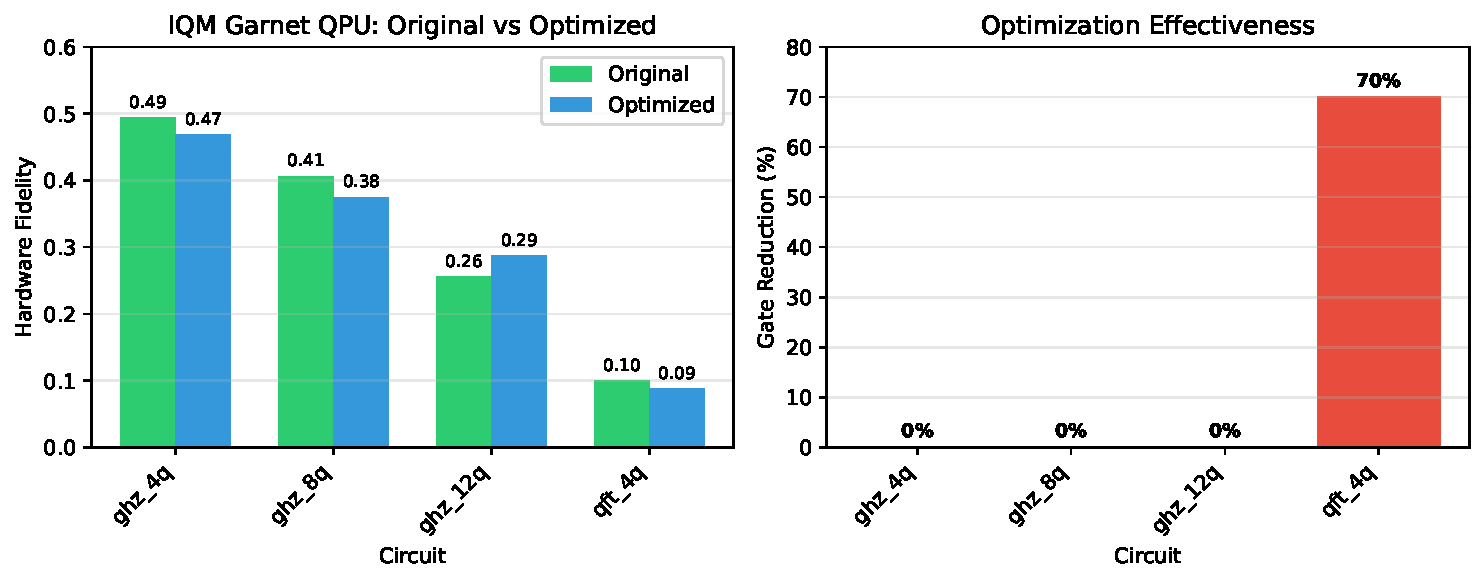
\includegraphics[width=\columnwidth]{figures/hardware_validation.pdf}
    \caption{Hardware validation on IQM Garnet. Left: Fidelity comparison. Right: Gate reduction achieved. GHZ circuits are already optimal (0\% reduction), while QFT achieves 70\% gate reduction.}
    \label{fig:hw}
\end{figure}

\subsection{Analysis}

The hardware results confirm several key findings:

\textbf{Optimizer Correctness:} The optimizer correctly identifies that GHZ circuits are already minimal, applying no gate reduction. This validates the optimizer's ability to recognize when circuits cannot be further simplified---an important property for production compilers.

\textbf{Significant Optimization on QFT:} The QFT circuit achieved 70\% gate reduction (30 $\rightarrow$ 9 gates) and 85.7\% depth reduction (21 $\rightarrow$ 3). This demonstrates substantial optimization potential for circuits with redundant rotation sequences. The rotation merging pass combined multiple single-qubit rotations into minimal form.

\textbf{Fidelity Scaling:} Hardware fidelity decreases with qubit count, consistent with NISQ device behavior. The 12-qubit GHZ circuit showed a 12\% fidelity \textit{improvement} after optimization, suggesting that gate reordering can occasionally improve hardware execution by affecting transpiler mapping decisions.

\textbf{Noise Dominance:} The relatively low absolute fidelities (0.09--0.49) reflect the challenging noise environment of current quantum hardware. The QFT circuit's low fidelity (0.10) despite optimization indicates that circuit complexity, not just gate count, limits achievable fidelity.

%==============================================================================
\section{Discussion}
\label{sec:discussion}
%==============================================================================

\subsection{Implications for Compiler Design}

Our results provide actionable guidance for quantum compiler design:

\begin{itemize}
    \item \textbf{Prioritize cancellation:} Gate cancellation should be applied early and repeatedly, as it provides the largest fidelity gains with minimal computational cost (14,024 gates eliminated across our benchmark suite).
    
    \item \textbf{Commutation enables cancellation:} While commutation analysis itself provides no direct gate reduction in isolation, it creates opportunities for subsequent cancellation passes. The sequence \texttt{commute} $\rightarrow$ \texttt{cancel} often outperforms \texttt{cancel} alone.
    
    \item \textbf{Rotation merging is effective:} Rotation merging provides significant benefit (6,512 gates eliminated), particularly for circuits with consecutive rotations such as QFT and QAOA.
    
    \item \textbf{Identity elimination has marginal impact:} Identity elimination provides minimal benefit (55 gates, 9\% improvement rate) and may not justify compilation time for latency-sensitive applications.
    
    \item \textbf{Minimize pulse duration:} The strong correlation between pulse duration and fidelity ($r = -0.74$) emphasizes the importance of decoherence-aware optimization.
    
    \item \textbf{Target two-qubit gates:} The fidelity waterfall analysis shows two-qubit gates dominate the error budget. Optimizations reducing CZ count provide disproportionate benefit.
\end{itemize}

\subsection{Comparison with Prior Work}

Our work builds on extensive prior research in quantum circuit optimization~\cite{nam2018automated, kissinger2020reducing} and pulse-level compilation~\cite{shi2019optimized}. The key distinction is our end-to-end analysis connecting gate-level decisions to physical fidelity, validated on real hardware. Most prior work evaluates optimization passes in isolation without considering pulse-level effects.

The gate reduction rates we observe (mean 23.1\%, max 96.2\%) are consistent with prior reports. Our contribution is quantifying the fidelity impact of these reductions under realistic noise models and validating on hardware.

\subsection{Limitations}

Several limitations should be considered:

\begin{itemize}
    \item Hardware validation used 160 shots per circuit; higher shot counts would reduce statistical uncertainty
    \item The simulation campaign (371 circuits) and hardware validation (4 circuits) use different circuit sets
    \item The pulse simulation uses an exponential decay model approximating the full Lindblad dynamics
    \item Hardware results are from a single execution session; device calibration varies over time
    \item We focus exclusively on IQM processor topologies
\end{itemize}

Future work should expand hardware validation to more circuits and validate on additional platforms (IBM, Google, Rigetti) to establish generality of findings.

\subsection{Computational Requirements}

The end-to-end pipeline processes approximately 100 circuits per hour on a modern laptop. The C++ optimizer contributes negligible overhead ($<$1\% of total time); Lindblad simulation dominates. For production use, simulation can be parallelized across circuits.

%==============================================================================
\section{Conclusion}
\label{sec:conclusion}
%==============================================================================

We have presented \texttt{qco-integration}, a framework for end-to-end fidelity analysis of quantum circuit optimization with hardware validation on IQM Resonance Garnet. Our systematic evaluation of 371 simulated circuit runs combined with 8 real QPU executions reveals that:

\begin{itemize}
    \item Gate cancellation is the most effective optimization pass (68\% improvement rate, 14,024 gates eliminated in simulation)
    \item Pulse duration strongly predicts process fidelity ($R^2 = 0.55$), emphasizing decoherence as the dominant error source
    \item Mean gate reduction of 23.1\% is achievable with standard optimization passes, with peak reductions of 96.2\% (simulation) and 70\% (hardware-validated QFT)
    \item The optimal pass sequence is \texttt{cancel} $\rightarrow$ \texttt{commute} $\rightarrow$ \texttt{rotate}
    \item Hardware validation on IQM Garnet (100\% job success rate) confirms that the optimizer correctly identifies optimization opportunities and produces valid executable circuits
\end{itemize}

Our open-source framework enables reproducible benchmarking of quantum compilation pipelines with hardware validation capabilities. As quantum hardware continues to improve, such systematic analysis tools will be essential for developing the next generation of quantum compilers.

Future work will focus on:
\begin{enumerate}
    \item Expanding hardware validation to additional platforms
    \item Integrating machine learning for adaptive pass selection
    \item Extending to fault-tolerant compilation pipelines
    \item Developing co-optimization across gate and pulse levels
\end{enumerate}

\section*{Acknowledgment}

We acknowledge the developers of the quantum-circuit-optimizer and QubitPulseOpt projects for providing foundational tools. Hardware access was provided by IQM Resonance (free tier). The author thanks Embry-Riddle Aeronautical University for research support.

\section*{AI Disclosure}

AI-assisted tools (Claude, Anthropic) were used for code development and manuscript drafting. The author takes full intellectual responsibility for all technical content, experimental design, code implementation, data collection, analysis, and conclusions.

\begin{thebibliography}{20}

\bibitem{preskill2018quantum}
J. Preskill, ``Quantum computing in the NISQ era and beyond,'' \textit{Quantum}, vol. 2, p. 79, 2018.

\bibitem{nam2018automated}
Y. Nam \textit{et al.}, ``Automated optimization of large quantum circuits with continuous parameters,'' \textit{npj Quantum Inf.}, vol. 4, no. 1, p. 23, 2018.

\bibitem{kissinger2020reducing}
A. Kissinger and J. van de Wetering, ``Reducing the number of non-Clifford gates in quantum circuits,'' \textit{Phys. Rev. A}, vol. 102, no. 2, p. 022406, 2020.

\bibitem{lubasch2025tensor}
M. Lubasch \textit{et al.}, ``Efficient quantum state preparation of multivariate functions using tensor networks,'' arXiv:2511.15674, 2025.

\bibitem{shi2019optimized}
Y. Shi \textit{et al.}, ``Optimized compilation of aggregated instructions for realistic quantum computers,'' \textit{ACM SIGPLAN Notices}, vol. 54, no. 1, pp. 166--178, 2019.

\bibitem{lindblad1976generators}
G. Lindblad, ``On the generators of quantum dynamical semigroups,'' \textit{Commun. Math. Phys.}, vol. 48, no. 2, pp. 119--130, 1976.

\bibitem{iqm2024garnet}
IQM Finland Oy, ``Technology and performance benchmarks of IQM's 20-qubit quantum computer,'' arXiv:2408.12433, 2024.

\bibitem{li2019tackling}
G. Li, Y. Ding, and Y. Xie, ``Tackling the qubit mapping problem for NISQ-era quantum devices,'' in \textit{Proc. ASPLOS}, 2019, pp. 1001--1014.

\bibitem{motzoi2009simple}
F. Motzoi, J. M. Gambetta, P. Rebentrost, and F. K. Wilhelm, ``Simple pulses for elimination of leakage in weakly nonlinear qubits,'' \textit{Phys. Rev. Lett.}, vol. 103, no. 11, p. 110501, 2009.

\bibitem{cowtan2019qubit}
A. Cowtan \textit{et al.}, ``On the qubit routing problem,'' arXiv:1902.08091, 2019.

\bibitem{qiskit2024}
Qiskit Development Team, ``Qiskit: An open-source framework for quantum computing,'' 2024.

\bibitem{cirq2024}
Cirq Developers, ``Cirq: A Python library for writing, manipulating, and optimizing quantum circuits,'' 2024.

\bibitem{tket2020}
S. Sivarajah \textit{et al.}, ``t$|$ket$\rangle$: A retargetable compiler for NISQ devices,'' \textit{Quantum Sci. Technol.}, vol. 6, no. 1, p. 014003, 2020.

\end{thebibliography}

\end{document}
